% -----------------------------------------------------------------
%		 				 Dynamic Models
% -----------------------------------------------------------------
\begin{tcolorbox}[colback=green!5!white,colframe=green!75!black,title=\textbf{Linear Time Invariant (LTI) Systems}]
With A, B, C, D are matrices
\begin{align*}
	\dot x &= Ax+Bu \quad y = Cx+Du \\
	G(s) &= C (sI-A)^{-1} B+D
\end{align*}

\textbf{LTI sytems as Input-Output Models:}
\begin{align*}
	G(S) = \frac{ b_0 + b_1s+...+b_ns^n }{ a_0+a_1s+...+a_{n-1}s^{n-1}+s^n } 
\end{align*}
\end{tcolorbox}

\begin{tcolorbox}[colback=green!5!white,colframe=green!75!black,title=\textbf{Deterministic Models}]
\todo[inline]{Hier fehlt noch etwas}
\begin{flalign*}
	y(k)=M(k;U,x_{init},p) 
\end{flalign*}

\begin{flalign*}
	&\textbf{Finite Impulse Response (FIR): } &\\
	&G(z) = b_0 + b_1z^{-1} + \cdots + b_{n_b}z^{-n_b} = \frac{b_0z^{n_b} + b_1z^{n_b-1} + \cdots + b_{n_{b}}}{z^{n_b}+0+ \cdots +0} &\\
	&\textbf{Auto Regressive Models with Exogenus Inputs (ARX): } &\\
	&G(z) = \frac{b_0z^n + b_1z^{n-1} + \cdots + b_n}{a_0z^n + a_1z^{n-1} + \cdots + a_n}&
\end{flalign*}
\end{tcolorbox}

\begin{tcolorbox}[colback=green!5!white,colframe=green!75!black,title=\textbf{Stochastik Models}]
\textbf{Model with measurement Noise:} \\ \(y(k)=M(k;U,{ x }_{ init },p)+\varepsilon(k)\) \\
\textbf{Liniar In the Parameters models (LIP):}
\begin{equation*}
y(k) = \sum_{i= 1}^{d}\theta_i\phi_i(u(k)...,y(k-1),...)+\epsilon(k)
\end{equation*}
$\rightarrow y(k) = \varphi(k)^T\theta + \epsilon(k)$ for $\varphi = (phi_1(\cdot),...,\phi_d(\cdot))$ \\
\textbf{LIP-LTI Models with Equation Errors (ARX)}\\
combining best of two worlds (LTI and LIP)
\begin{equation*}
a_0y(k)+...+a_{n_{a}}y(k-n_a) = b_0u(k)+...+b_{n_{b}}u(k-n_b)+\epsilon(k)
\end{equation*}
\end{tcolorbox}

\begin{tcolorbox}[colback=green!5!white,colframe=green!75!black,title=\textbf{Model with Input and Output Errors}] 
	\begin{equation*}
	y(k)=M(k;U + \varepsilon_{N}^{u}, x_{init}, p) + \varepsilon^y (k)
	\end{equation*}
	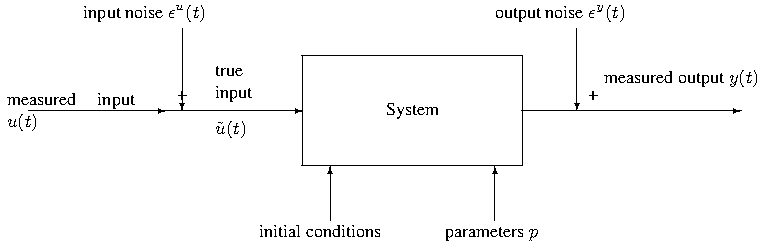
\includegraphics[width=\textwidth]{model.pdf}
\end{tcolorbox}

\begin{tcolorbox}[colback=green!5!white,colframe=green!75!black,title=\textbf{Pure Output Error (OE) Minimization}]
\begin{equation*}
	\theta_{ML} =\underset{\theta}{min} \sum_{k=1}^{N} (y(k)-M(k;U, x_{init} p))^2
\end{equation*}

\textbf{Output Error Minimization for FIR Models:}
\begin{flalign*}
	y(k) &= (u(k), u(k-1), \cdots , u(k-n_{n_b})) \cdot \theta +\varepsilon(k) &\\
	&= \underset {\theta}{min} \sum_{k=n_{b}+1}^{N} (y(k)-(u(k), u(k-1), \cdots , u(k-n_{n_b})) \cdot \theta)^2 &
\end{flalign*}

\textbf{Models with Input and Output Errors:}
\begin{flalign*}
	& \underset{\theta}{arg\,min} \sum_{k-1}^{N} \frac{1}{\sigma_{y}^{2}} (y(k)-M(k;U+ \epsilon_{N}^{u},x_{init},p))^2 + \frac{1}{\sigma_{u}^{2}} (\epsilon_u (k))^2 & \\
	& \underset{\theta}{arg\,min} \sum_{k-1}^{N} \frac{1}{\sigma_{y}^{2}} (y(k)-M(k;\tilde U, x_{init}, p))^2 + \frac{1}{\sigma_{u}^{2}} (u(k)-\tilde u(k) )^2 &
\end{flalign*}
\end{tcolorbox}